\documentclass[12pt]{article}
\usepackage[utf8]{inputenc}
\usepackage{graphicx}
\graphicspath{ {./images/} } % Uncomment
\usepackage[
top=2cm,
bottom=2cm,
left=2cm,
right=2cm,
headheight=17pt, % as per the warning by fancyhdr
includehead,includefoot,
heightrounded, % to avoid spurious underfull messages
]{geometry} 
\geometry{a4paper}
\usepackage{fancyhdr}
\usepackage{booktabs}

% Lecture Name, exercise number, group number/members
\newcommand{\lecture}{GPU Computing}
\newcommand{\exercise}{Exercise 5}
\newcommand{\groupnumber}{gpucomp03}
\newcommand{\groupmembersshort}{Benjamin Maier, Daniel Barley, Laura Nell}
\newcommand{\groupmemberslist}{Benjamin Maier\\Daniel Barley\\Laura Nell}
\newcommand{\duedate}{December 15th, 09:00}



\fancyhf{}
\fancyhead[L]{\groupnumber}
\fancyhead[R]{\textsc{\groupmembersshort}}
\fancyfoot[C]{\lecture: \exercise}
\fancyfoot[R] {\thepage}
\renewcommand{\headrulewidth}{0.4pt}
\renewcommand{\footrulewidth}{0.4pt}
\pagestyle{fancy}

\begin{document}
	\begin{titlepage}
		\centering

		{\scshape\LARGE Heidelberg University\\Institute for Computer Engineering (ZITI) \par}
		\vspace{1.5cm}
		{\scshape\Large Master of Science Computer Engineering \par}
		\vspace{0.5cm}
		{\scshape\Large \lecture \par}
		\vspace{1.5cm}
		{\huge\bfseries \exercise \par}
		\vspace{2cm}
		{\Large \groupnumber \itshape \\ \vspace{30pt} \groupmemberslist \par}
		\vfill
		
		
		% Bottom of the page
		{\large Due date \duedate \par}
	\end{titlepage}

\setcounter{section}{5}

\subsection{Reading}
\subsubsection*{The GPU Coputing Era}
Because of the still increasing demand for faster and higher-definition graphics, the development of increasingly parallel and programmable GPUs has not stopped yet. Using the example of Nvidia GPUs, the evolution of GPU computing and its parallel computing model as well as the benefit of CPU+GPU coprocessing are described with proof by example application performance speedups. In particular, the focus of the, at that time, state of the art architectures lies on the one hand on the CUDA scalable parallel architecture, on the other hand, regarding computing architectures, on the Fermi scalable computing architecture.\\\\
The Fermi computing architecture enables a raise in throughput by several novel features like its streaming multiprocessors introducing a memory model using fast on-chip shared memory or ECC memory protection.\\
The main conclusion is, that CPU+GPU coprocessing enables much more efficient execution of almost all kinds of algorithms by using the CPU, which is latency optimized, for serial parts of the code and the GPU, which is throughput optimized, for parallel parts of the code. This fits perfectly for the CUDA programming model, which is able to launch a series of parallel kernels from a single sequential control thread.\\\\
The CUDA programming model is still widely used in today's applications due to its specialization on parallel computing. It is also still state of the art to extend CPU+GPU coprocessing for time consuming applications, although with further developed computing architectures. Therefore, we accept the paper and its content.

\vspace{10pt}

\newpage
\subsection{Matrix Multiply - GPU naive version}

\begin{figure}[htpb]
	\centering
	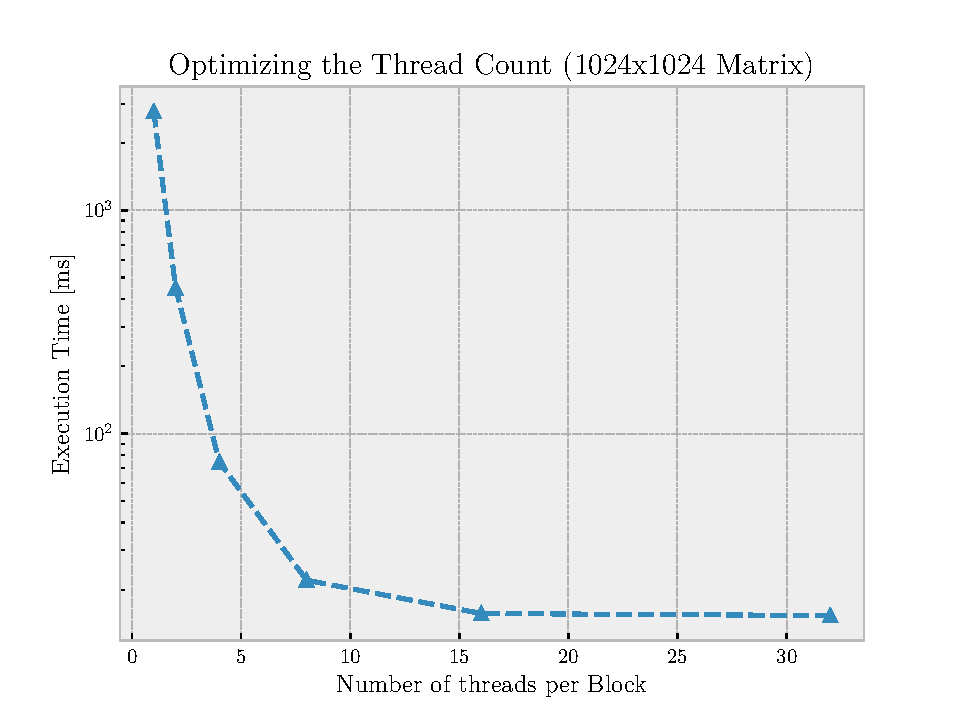
\includegraphics[width=1\linewidth]{../eval/thread_count.pdf}
	\caption{The thread per block count was varied between 1 and 32.
The best performance is unsurprisingly achieved when using the maximum of 32
threads per block. This is in line with previous observations that less threads
doing smaller tasks limits performance significantly.}
	\label{fig:../eval/thread_count}
\end{figure}

\begin{figure}[htpb]
	\centering
	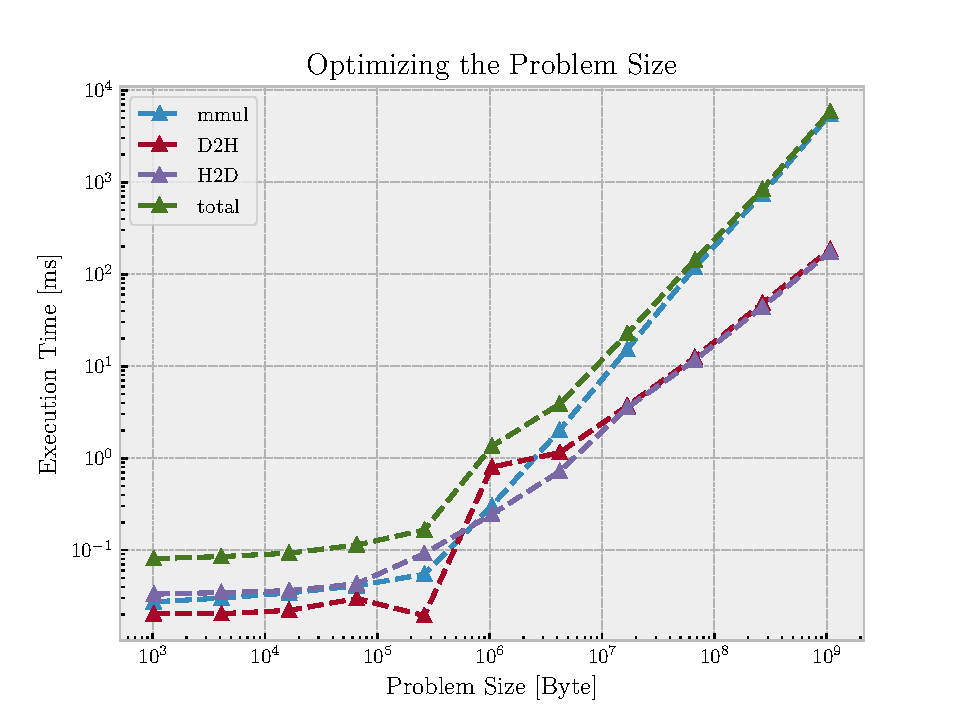
\includegraphics[width=1\linewidth]{../eval/problem_size.pdf}
	\caption{Using the optimal count of 32 threads the problem size was varied
and the latencies due to data movement and computation compared.
For smaller problem sizes data movement is far too expensive.
Only when reaching a few mega bytes the computation amortizes the movement of data}%
	\label{fig:../eval/problem_size}
\end{figure}

\newpage
\subsection{Matrix Multiply - GPU version using shared memory}

\begin{figure}[htpb]
	\centering
	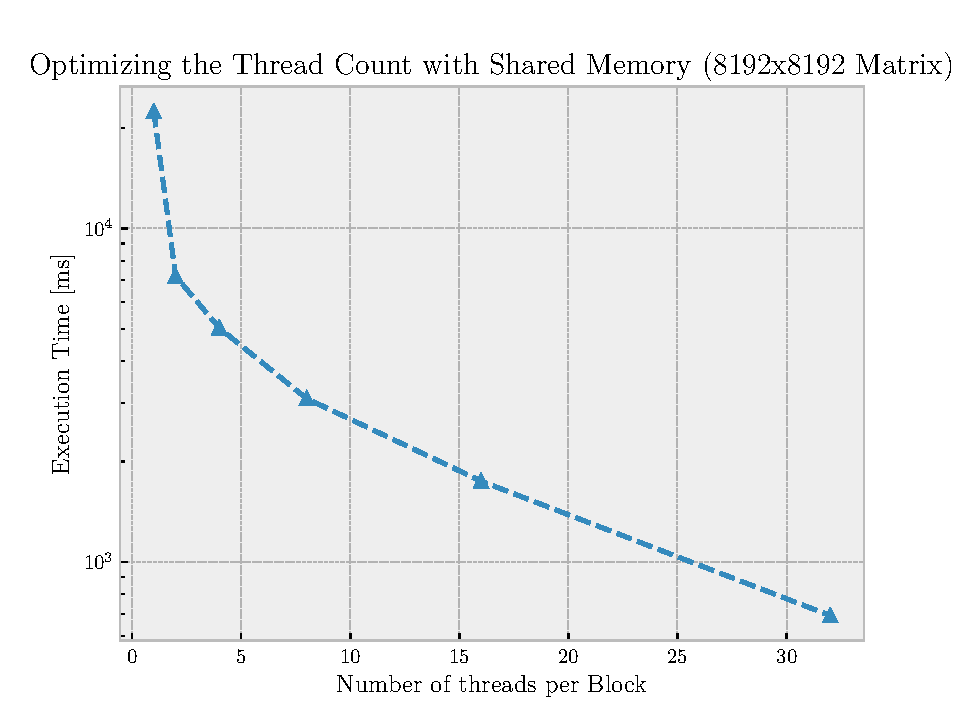
\includegraphics[width=1\linewidth]{../eval/sh_thread_count.pdf}
	\caption{The same as in the previous task was done for the shared memory
	optimized version. Again the maximum number of threads is optimal.
Additionally to the computation more threads mean a faster collaborative
load into shared memory.}%
	\label{fig:../eval/sh_thread_count}
\end{figure}

\begin{figure}[htpb]
	\centering
	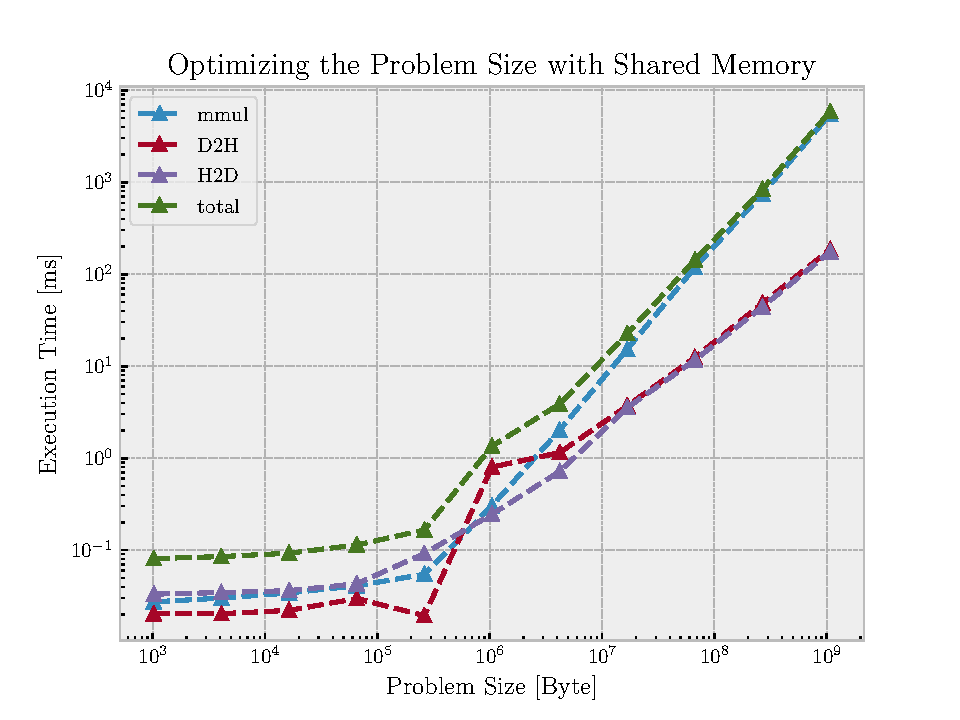
\includegraphics[width=1\linewidth]{../eval/sh_problem_size.pdf}
	\caption{Same as the naïve version}%
	\label{fig:../eval/sh_problem_size}
\end{figure}

\begin{figure}[htpb]
	\centering
	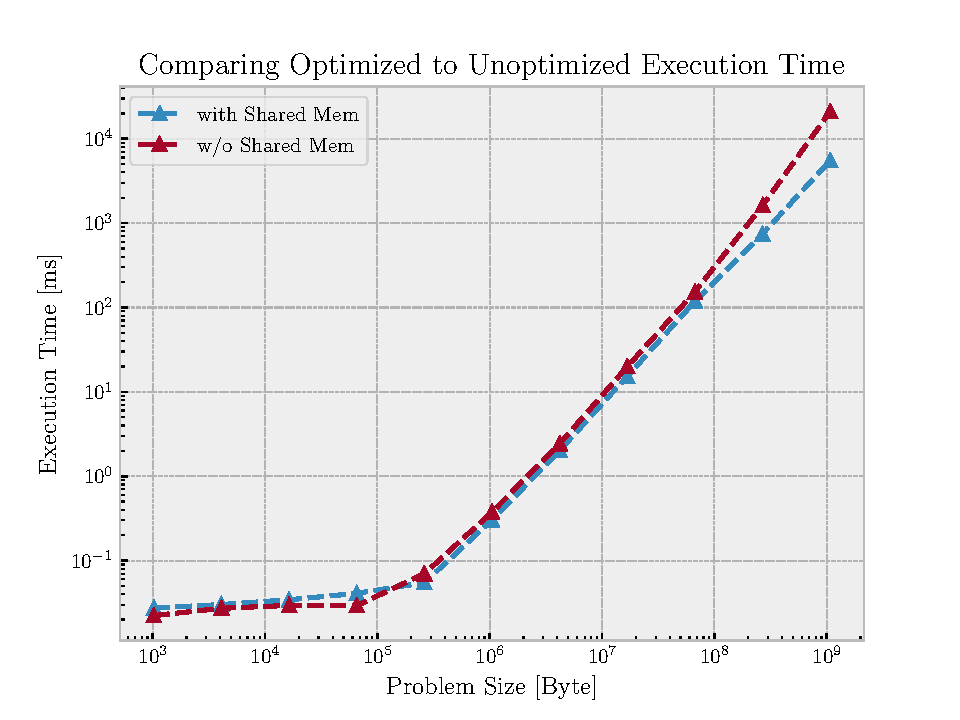
\includegraphics[width=1\linewidth]{../eval/compare.pdf}
	\caption{Comparing execution times of the naïve and optimized versions
	reveals that for small problem sizes there is no notable difference.
The naïve version even out performs the shared memory version probably due to
the data movement and synchronization overhead introduced.}%
	\label{fig:../eval/compare}
\end{figure}

\begin{figure}[htpb]
	\centering
	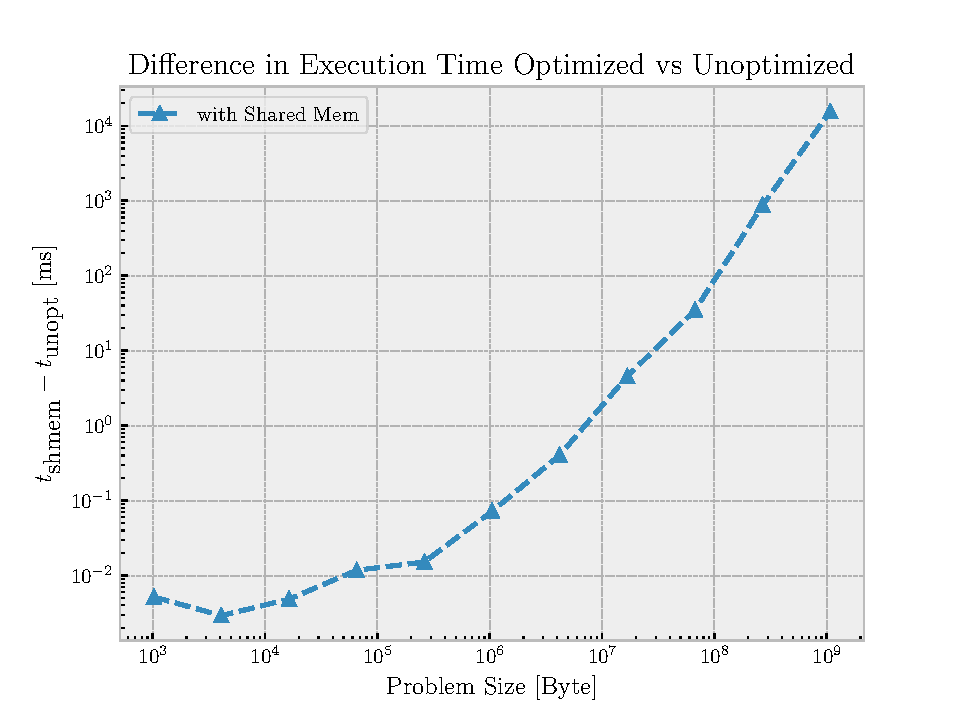
\includegraphics[width=1\linewidth]{../eval/diff.pdf}
	\caption{Difference in execution time visualized. The shared memory
	optimized matrix multiply starts to outperform the naïve version in
the hundreds of mega bytes.}%
	\label{fig:../eval/diff}
\end{figure}


\begin{table}[htpb]
	\centering
	\caption{
		Speedups acheived for 1024x1024 (largest value tested on CPU)
}
	\label{tab:k}
	\begin{tabular}{ll}
		\toprule
		Program Version & Speedup \\
		\midrule
		unoptimized excl. data movement & 301\\
		unoptimized inc. data movement & 154\\
		optimized excl. data movement & 361\\
		optimized inc. data movement & 188\\
		\bottomrule
	\end{tabular}
\end{table}

\newpage
\subsection{Willingness to present}
Hereby, we declare our will to present the results presented in the former sections.


\end{document}
